% !TEX root=../main.tex

\section{Results}\label{sec:results}

To test our implementation, we used the EuRoC datasets~\cite{Burri2016}.
We selected an easy case and hard case of the EuRoC datasets to test the algorithm, MH\_02 and MH\_04.
Timing data for the new modules in Anticipated VINS-Mono is given in Table~\ref{tab:timing}.
Running this algorithm against VINS-Mono without anticipated feature selection would not be a good comparison since VINS-Mono can select up to 150 features and would be expected to do better than any method selecting fewer features.
In order to have a benchmark to test the attention algorithm against, we made two test cases: \textit{quality} and \textit{random}.
In \textit{quality}, we run VINS-Mono without the anticipation algorithm, but limit the maximum features it can select to the size of $\kappa$ we use for the attention algorithm.
For \textit{random}, we conduct feature selection randomly, choosing at random from the set of new features seen to satisfy the same $\kappa$ constraint.
The results are given in Figure~\ref{tab:results}.

We can see that Anticipated VINS-Mono does better than both \textit{quality} and \textit{random} in certain cases.
With the 10 features on the easier dataset, Anticipated VINS-Mono does better than \textit{random} and better than \textit{quality} as quality ended up being unstable.
With 30 features, Anticipated VINS-Mono does better than \textit{quality} and \textit{random} again, with lower absolute translational error (ATE) and rotational translational error (RTE).
However, Anticipated-VINS Mono does not perform well on MH\_05, the more difficult dataset, whereas \textit{quality} still produces a meaningful pose estimate.

There are a few reasons that could explain why Anticipated VINS-Mono does not work perfectly.
Calculating $\OmegakkH^\text{PRIOR}$ was not implemented in the algorithm itself due to time constraints in retrieving it from VINS-Mono backend.
Including $p_l$ was also not included due to time constraints.
At times, the processed poses showed that the pose (and error) was unstable and kept increasing (e.g., in Anticipated VINS-Mono run on MH\_05 with 30 features).
Moreover, we did not look at the VINS-Mono back end optimizer, and it is possible that Anticipated VINS-Mono could be improved there.

Parameters used are given in Table~\ref{tab:parameters} with a timing summary in Table~\ref{tab:timing}\footnote{Video results can be seen at \url{https://www.youtube.com/watch?v=OOzhGPaxFd8}.}.

\begin{figure}
\centering
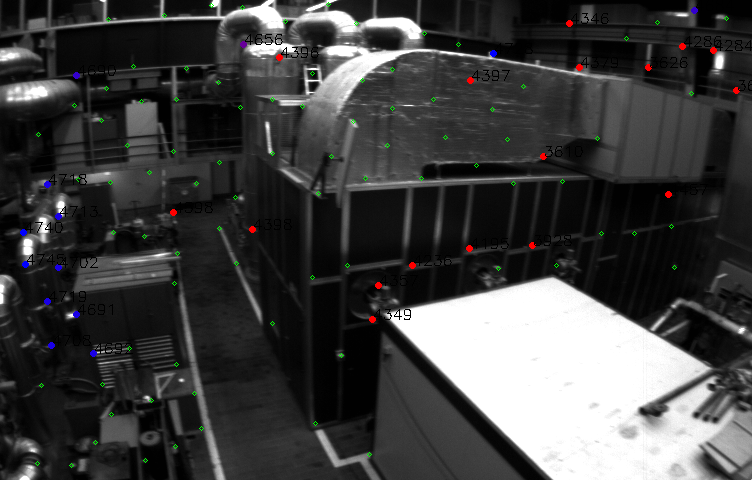
\includegraphics[width=\columnwidth]{mh5_leftyaw} 
\caption{Snapshot of EuRoC \texttt{MH\_05\_difficult} during a sharp left turn. Possible selections (new detections) are shown in green, selected features in blue, and tracked features in red. Notice how \texttt{Anticipated VINS-Mono} selects the majority of its features on the left side of the frame.}
\label{fig:architecture} 
\end{figure}

\begin{figure}
	\centering
	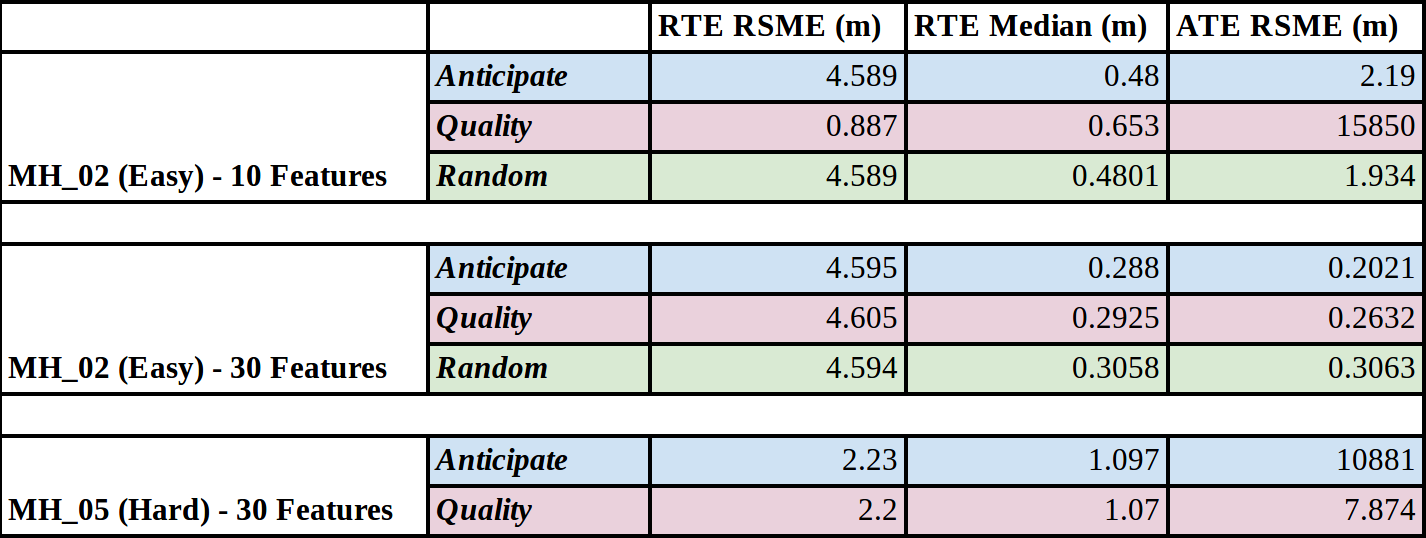
\includegraphics[width=\columnwidth]{tableVNAVresults.png} 
	\caption{Results of Anticipated VINS-Mono on EuRoC datasets against benchmarks \textit{quality} and \textit{random}}
	\label{tab:results} 
\end{figure}

\begin{table}[h]
\centering
\caption{Parameters}
\begin{tabular}{ll}
    \toprule
    Parameter & Value \\
    \midrule
    Frame rate & 10 Hz \\
    Horizon & 10 frames \\
    Max features to detect & 150 \\
    Features to maintain, $\bar{\kappa}$ & 30 \\
    \bottomrule
\end{tabular}
\label{tab:parameters}
\end{table}

\begin{table}[h]
\centering
\caption{Timing Statistics on EuRoC MH\_05\_difficult}
\begin{tabular}{clc}
    \toprule
    Thread & Component & Time (ms) \\
    \midrule
    1 & Feature Tracker & 18 \\
    \midrule
    2 & Feature Selector & 9 \\
      & Windowed Optimization (1 sec) & 30 \\
    \bottomrule
\end{tabular}
\label{tab:timing}
\end{table}